\documentclass[tikz,border=8pt]{standalone}
\usepackage[T1]{fontenc}
\usepackage{lmodern}
\usetikzlibrary{arrows.meta,positioning,fit,backgrounds}

\begin{document}
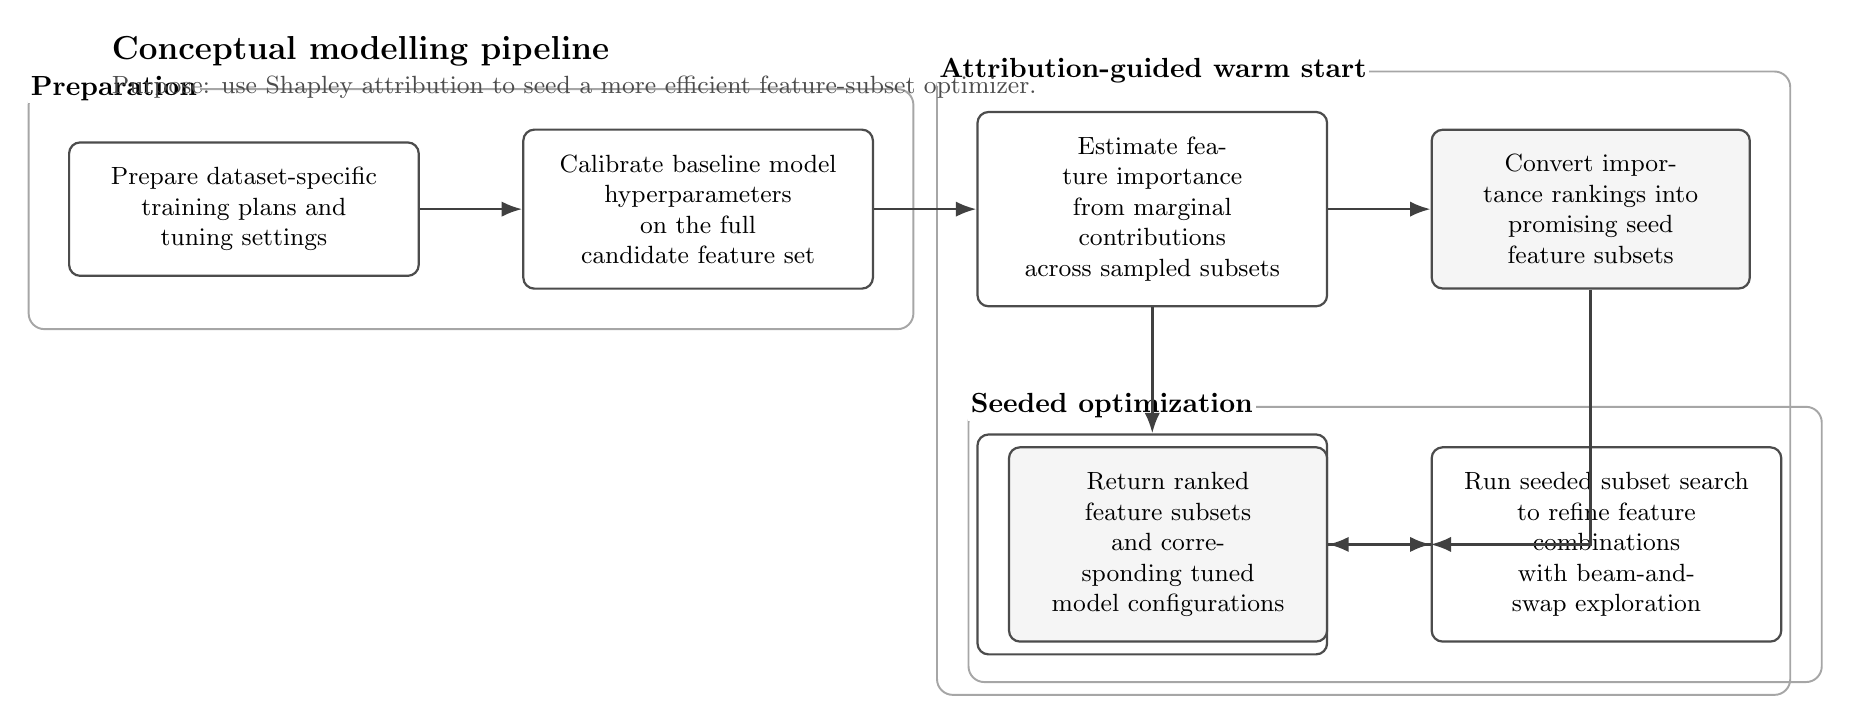
\begin{tikzpicture}[
    font=\small,
    >=Latex,
    flow/.style={draw=black!75, line width=0.95pt, -{Latex[length=2.6mm]}},
    block/.style={
        draw=black!70,
        rounded corners=1.4mm,
        line width=0.8pt,
        fill=white,
        minimum height=10mm,
        text width=38mm,
        align=center,
        inner sep=3.2mm
    },
    artifact/.style={
        block,
        fill=black!4,
        text width=34mm
    },
    stagebox/.style={
        draw=black!35,
        rounded corners=2mm,
        line width=0.7pt,
        inner sep=5mm
    },
    stagelabel/.style={
        font=\bfseries,
        anchor=west,
        fill=white,
        inner sep=1pt
    }
]

\node[anchor=west, font=\bfseries\large] (title) at (0, 4.9)
{Conceptual modelling pipeline};
\node[anchor=west, text=black!70] at (0, 4.45)
{Purpose: use Shapley attribution to seed a more efficient feature-subset optimizer.};

\node[block] (setup) at (1.8, 2.9)
{Prepare dataset-specific\\training plans and tuning settings};

\node[block, right=13mm of setup] (fullcv)
{Calibrate baseline model\\hyperparameters on the full\\candidate feature set};

\node[block, right=13mm of fullcv] (shapley)
{Estimate feature importance\\from marginal contributions\\across sampled subsets};

\node[artifact, right=13mm of shapley] (seeds)
{Convert importance rankings into\\promising seed feature subsets};

\node[block, below=16mm of shapley] (subsetcv)
{Retune the model on the best\\attribution-derived subsets to\\stabilize regularization choices};

\node[block, right=13mm of subsetcv] (optimizer)
{Run seeded subset search\\to refine feature combinations\\with beam-and-swap exploration};

\node[artifact, left=13mm of optimizer] (output)
{Return ranked feature subsets\\and corresponding tuned\\model configurations};

\draw[flow] (setup) -- (fullcv);
\draw[flow] (fullcv) -- (shapley);
\draw[flow] (shapley) -- (seeds);
\draw[flow] (seeds) |- (optimizer);
\draw[flow] (shapley) -- (subsetcv);
\draw[flow] (subsetcv) -- (optimizer);
\draw[flow] (optimizer) -- (output);

\begin{scope}[on background layer]
    \node[stagebox, fit=(setup)(fullcv),
        label={[stagelabel]north west:Preparation}] {};
    \node[stagebox, fit=(shapley)(seeds)(subsetcv),
        label={[stagelabel]north west:Attribution-guided warm start}] {};
    \node[stagebox, fit=(optimizer)(output),
        label={[stagelabel]north west:Seeded optimization}] {};
\end{scope}

\end{tikzpicture}
\end{document}
